% Recitation 11: Poisson Brackets recap
% Lec. 14: Scattering Amplitudes
% Lec. 15: Rutherford Scattering
% Lec. 16: Principle Axes of Rotation / Rigid Body Motion
% Action-Angle Variables / Final Summary / Rec. 17

\chapter{Poisson Brackets, Scattering, Rigid Body Motion, and Action-Angle Variables}

%%==========================================================================
\section{SHO Example (Recitation 11: Poisson Brackets Recap)}
%%==========================================================================

We showed in class that $[u,v]_{q,p} = [u,v]_{Q,P}$.

\subsection*{Reproof}

For $f(q,p,t)$,
\begin{align*}
    \dv{f}{t} &= \pdv{f}{t} + \sum_k \left(\pdv{f}{q_k}\dot{q}_k + \pdv{f}{p_k}\dot{p}_k\right) \\
              &= \pdv{f}{t} + \sum_k \left(\pdv{f}{q_k}\pdv{H}{p_k} - \pdv{f}{p_k}\pdv{H}{q_k}\right) \\
              &= \pdv{f}{t} - [f, H]
\end{align*}

\subsection{SHO Example (1D)}

The Hamiltonian for the 1D SHO is:
\[
    H = \frac{p^2}{2m} + \frac{1}{2}m\omega^2 q^2
\]

Recall from last time, with the canonical transformation:
\[
    \begin{cases}
        p = a(P)\cos Q \\
        q = \dfrac{a(P)}{m\omega}\sin Q
    \end{cases}
    \implies a(P) = \sqrt{2Pm\omega}
\]

But can we find $a(P)$ with Poisson brackets?

We know $[q,q]_{Q,P} = 0$, $[P,P]_{Q,P} = 0$, and we require:
\[
    [q,p]_{Q,P} = \pdv{q}{Q}\pdv{p}{P} - \pdv{q}{P}\pdv{p}{Q}
    = \frac{a(P)}{m\omega}\cos^2 Q \cdot a'(P) + \frac{a'(P)}{m\omega}\sin^2 Q \cdot a(P)
    = \frac{a\,a'}{m\omega} = 1
\]

\textit{Why do we check this?} This confirms the transformation is canonical.

Therefore:
\[
    a(P)\,\pdv{a}{P} = m\omega
    \implies \int a\,da = \int m\omega\,dP
    \implies \frac{a^2}{2} = m\omega P
    \implies \boxed{a = \sqrt{2m\omega P}}
\]

\subsection{Poisson Brackets are Invariant Under Canonical Transformations}

\textbf{Method 1:} (statement only, details omitted)

%%==========================================================================
\chapter{Scattering Amplitudes}
%%==========================================================================

% Lec. 14, Monday January 27, 2025

\begin{itemize}
    \item Goal: predict scattering angle.
    \item First we ignore all long-range interactions.
\end{itemize}

\section{Setup}

\begin{figure}[H]
\begin{center}
\begin{tikzpicture}[scale=0.95, >=Stealth]
  % Target
  \fill[gray!40] (3.5,0) circle[radius=0.18];
  \node[above right] at (3.7,0.1) {$M$};
  % Incoming particle trajectory
  \draw[->,thick,blue] (0,0.6) -- (2.8,0.6);
  \node[above,blue,scale=0.85] at (1.0,0.6) {$\vect{p}_i$};
  % Impact parameter b
  \draw[<->,gray] (0,0) -- (0,0.6) node[midway,left]{$b$};
  \draw[dashed,gray] (0,0) -- (3.5,0);
  % Scattered trajectory
  \draw[->,thick,red] (3.5,0) -- ++(35:2.0);
  \node[right,red,scale=0.85] at (5.2,1.15) {$\vect{p}_f$};
  % Scattering angle theta
  \draw (3.5,0) ++(0:0.8) arc[start angle=0,end angle=35,radius=0.8];
  \node[right,scale=0.85] at (4.35,0.25) {$\theta$};
  % Asymptotic dashed lines
  \draw[dashed,gray] (2.0,0.6) -- (4.0,0.6);
\end{tikzpicture}
\end{center}
\caption{Scattering setup. A particle with initial momentum $\vect{p}_i$ and impact parameter $b$ (perpendicular distance from target centre) scatters through angle $\theta$ off a heavy target $M$.}
\label{fig:scattering_setup}
\end{figure}

\begin{itemize}
    \item $\theta$: scattering angle --- direction between initial and final momentum.
    \item $M$: $M \gg m$.
    \item $b$: impact parameter --- vertical displacement of a particle's initial position relative to a line going through the center of the sphere, in the $\vect{p}_i$ direction.
    \item $\alpha$ is the same on both sides because the \textbf{perp} component of momentum is conserved.
\end{itemize}

\textbf{Scenario:} There is a uniformly distributed beam of point particles of total radius much bigger than the target source ($\to 0$).

\section{Differential Cross Section}

\begin{figure}[H]
    \centering
    \caption{Differential cross section geometry. A solid angle element $d\Omega$ captures particles scattered into that region.}
\end{figure}

Define $\dfrac{d\sigma}{d\Omega}$ such that $\left(\dfrac{d\sigma}{d\Omega}\right)\Delta\Omega$ is the ratio of the scattering rate into $\Delta\Omega$ (differential element of solid angle) divided by the luminosity of the beam $L$.

\begin{itemize}
    \item $L$: number of incident beam particles per unit time and area.
    \item The total cross section:
    \[
        \sigma = \int \frac{d\sigma}{d\Omega}\,d\Omega = \frac{\text{total scattering rate}}{L}
    \]
    \item $\implies$ total scattering rate $= L\sigma$.
    \item Most scattering problems are azimuthally symmetric.
    \item If long-range interactions are turned off, then the scattering rate of incident beam particles for the range $(b,\, b+\Delta b)$ is:
    \[
        = L\left(\pi(b+\Delta b)^2 - \pi b^2\right) \approx L \cdot 2\pi b\,\Delta b
    \]
\end{itemize}

\begin{fact}[1]
There is a 1-to-1 mapping between $b$ and $\theta$.
\end{fact}

\begin{itemize}
    \item The rate of beam particles with impact parameter in $(b, b+\Delta b)$ must be the same as the rate of particles scattered into $\Delta\Omega$:
    \[
        L \cdot 2\pi b\,\Delta b = L\,\frac{d\sigma}{d\Omega}\,\Delta\Omega = L\,\frac{d\sigma}{d\Omega}\,2\pi\sin\theta\,d\theta
    \]
    \[
        \implies b\,\Delta b = \frac{d\sigma}{d\Omega}\sin\theta\,d\theta
    \]
    \item Note: $db/d\theta$ is negative (look at the first diagram), but $d\sigma/d\Omega$ must be positive. Therefore:
\end{itemize}

\begin{formula}[Differential Cross Section]
\[
    \boxed{\frac{d\sigma}{d\Omega} = \frac{b}{\sin\theta}\left|\frac{db}{d\theta}\right|}
\]
\end{formula}

From the top diagram:
\[
    b = R\sin\alpha,\quad \theta = \pi - 2\alpha \implies db = R\cos\alpha\,d\alpha,\quad d\theta = -2\,d\alpha
\]

\[
    \frac{d\sigma}{d\Omega} = \frac{R\sin\alpha}{\sin(\pi-2\alpha)}\left|\frac{db}{d\alpha}\frac{d\alpha}{d\theta}\right|
    = \frac{R\sin\alpha}{\sin(2\alpha)}\left|-\frac{R\cos\alpha}{2}\right| = \frac{R^2}{4}
\]

Scattering off a point particle off a sphere is \textbf{isotropic}; the probability of scattering into any region depends only on the size of that region.

To find the cross section:
\[
    \sigma = \int \frac{R^2}{4}\,d\Omega = \frac{R^2}{4}\cdot 4\pi = \pi R^2
\]

\section{Nuclear Reactions}

\begin{figure}[H]
    \centering
    \caption{U-235 fission. A neutron hits a U-235 nucleus, which splits into fragments and releases 3 more neutrons.}
\end{figure}

\begin{itemize}
    \item Mean free path:
    \[
        D = \frac{v_n}{L\sigma} = \frac{v_n}{\rho_U v_n \sigma} = \frac{1}{\rho_U \sigma}
        \quad\text{(mean distance between collisions)}
    \]
    \item Thus mean time between creation and fission is:
    \[
        T_f = \frac{5}{\sigma\rho_U v_n} \approx 10^{-8}\,\text{s}
    \]
    \item But the mean distance $\approx \sqrt{5}\,D = 7\,\text{cm}$.
\end{itemize}

\subsection*{Chain Reaction}

\[
    N(t + \Delta t) = N(t) + \frac{\Delta t}{T_f}\,N(t)(\nu p - 1)
\]
where $(\nu p - 1)$ counts the number of new neutrons that will eventually produce fission.

\[
    \implies \dv{N}{t} = \frac{(\nu p - 1)}{T_f}\,N
\]
\[
    \implies N(t) = N(0)\exp\!\left(\frac{(\nu p - 1)\,t}{T_f}\right)
\]

%%==========================================================================
\chapter{Rutherford Scattering}
%%==========================================================================

% Lec. 15, Tuesday January 28, 2025

\begin{itemize}
    \item Context: plum pudding model of the atom --- electrons could move around in positive ``goo''.
\end{itemize}

\subsection*{Rutherford Experiment}

\begin{figure}[H]
    \centering
    \caption{Rutherford's experimental setup: a radioactive source fires alpha particles through a thin foil target; a detector ring surrounds the setup to measure scattered particles.}
\end{figure}

\section{Scattering}

\begin{figure}[H]
    \centering
    \caption{Scattering trajectory. The particle asymptotes toward the regular (no interaction) scattering direction. At the point of closest approach the angle is $\alpha$ on each side (by time-reversal symmetry), and $\theta = \pi - 2\alpha$.}
\end{figure}

\begin{itemize}
    \item The particle asymptotes toward the regular (no interaction) scattering direction.
    \item Point of closest approach: at this point the momentum is perpendicular to $\hat{r}$.
    \item By time-reversal symmetry, $\alpha$ on the left equals $\alpha$ on the right.
    \item $U = \dfrac{k}{r}$ (compare to $-\dfrac{GMm}{r}$).
    \item Recall that for gravity, $\dfrac{\beta}{r} = 1 + \varepsilon\cos\phi$, where
    \[
        \beta = \frac{\ell^2}{mGMm} \longrightarrow \beta_{\text{electric}} = \frac{\ell^2}{km}
    \]
    \item We also have to change sign (will do later):
    \[
        \varepsilon = \sqrt{1 + \frac{2E\ell^2}{m(GMm)^2}} \implies \sqrt{1 + \frac{2E\ell^2}{mk^2}}
    \]
    \item Therefore:
    \[
        -\frac{\beta}{r} = 1 + \varepsilon\cos(\phi + \alpha)
    \]
    where $\alpha$ makes $r_{\min}$ (radius of closest approach).
    \item Take the point $r\to\infty$, $\phi\to\pi$:
    \[
        0 = 1 - \varepsilon\cos\alpha \implies \cos\alpha = \frac{1}{\varepsilon}
    \]
    (We use this to find $\alpha$ from $\varepsilon$ because $\varepsilon$ doesn't change, so you can use any point.)
    \item $E_{\text{initial}} = \dfrac{p_i^2}{2m}$, $\ell_{\text{init}} = bp_i$.
    \item Temporary variable: let $\gamma = \dfrac{k}{2E}$, so $\ell^2 = b^2\cdot 2mE = \dfrac{b^2 mk}{\gamma}$.
    \[
        \cos\alpha = \frac{1}{\sqrt{1 + \dfrac{2E\ell^2}{mk^2}}} = \frac{\gamma}{\sqrt{\gamma^2 + b^2}}
    \]
    \item Then we know $\tan\alpha = \dfrac{b}{\gamma} = \tan\!\left(\dfrac{\pi-\theta}{2}\right) = \cot\!\left(\dfrac{\theta}{2}\right)$.
    \[
        \frac{db}{d\gamma} = \frac{-1}{\sin^2\!\dfrac{\theta}{2}}\cdot\frac{d\theta}{2}
    \]
    \item Recall that if you have azimuthal symmetry:
\end{itemize}

\begin{align*}
    \frac{d\sigma}{d\Omega}
    &= \frac{b}{\sin\theta}\left|\frac{db}{d\theta}\right|
    = \frac{\gamma\cot(\theta/2)}{\sin\theta}\cdot\frac{\gamma}{2\sin^2(\theta/2)}
    = \frac{\gamma\cos(\theta/2)}{\sin\theta\cdot 2\sin^2(\theta/2)} \cdot \frac{1}{2\sin^2(\theta/2)}\\
    &= \frac{\gamma^2}{4\sin^4(\theta/2)}
\end{align*}

\begin{formula}[Rutherford Scattering Cross-Section]
\[
    \boxed{\frac{d\sigma}{d\Omega} = \frac{k^2}{(4E)^2\sin^4(\theta/2)}}
\]
\end{formula}

The only way you could get scattering if you concentrate the positive charge inside the atom.

\section{Energy Dissipation of a Charged Particle}

\begin{figure}[H]
    \centering
    \caption{A heavy particle $P$ moving with velocity $v$ through a medium of electrons.}
\end{figure}

Consider the rest frame of the particle $P$:
\begin{itemize}
    \item In this frame, electrons move toward $P$ with kinetic energy $E_e = \frac{1}{2}m_e v^2$.
    \item Assume $\theta \ll 1$:
    \[
        \frac{b}{\gamma} = \frac{2Eb}{k} = \cot\frac{\theta}{2} \approx \frac{2}{\theta}
        \quad\text{(small angle approximation)}
    \]
    \[
        \implies \theta \approx \frac{k}{Eb} = \frac{2k}{m_e v^2 b}
        \quad\text{(plug in initial energy)}
    \]
    \[
        \vect{p}_i^e = m_e v\,\hat{x} \implies \vect{p}_f^e = m_e v(\cos\theta\,\hat{x} + \sin\theta\,\hat{y})
        \approx m_e v(\hat{x} + \theta\,\hat{y})
    \]
    \[
        \implies \Delta\vect{p}_e = m_e v\theta\,\hat{y} \approx \frac{2k}{vb}\,\hat{y}
        \quad\text{(this is approximately the momentum that the proton loses)}
    \]
    \[
        \Delta E \approx -\frac{|\Delta p_e|^2}{2m_e} = -\frac{2k^2}{m_e v^2 b^2}
    \]
\end{itemize}

\begin{figure}[H]
    \centering
    \caption{Volume shell of thickness $db$ and width $dx$ around the particle trajectory, used to count electrons encountered.}
\end{figure}

\begin{align*}
    dE &= \left[\frac{-2k^2}{m_e v^2 b^2}\right]
         \cdot\left[\pi(b+\Delta b)^2 - \pi b^2\right]\Delta x
         \cdot\left[\frac{Z\rho}{Am_p}\right] \\
       &\approx \frac{-2k^2}{m_e v^2 b^2}\cdot 2\pi b\,\Delta b\,\Delta x
         \cdot\frac{Z\rho}{Am_p}
\end{align*}

where $Z$ is the number of electrons per atom, $A$ is the atomic mass (number of protons + neutrons), $m_p$ is the mass of the proton, and $\rho$ is the mass density.

\[
    \frac{d^2E}{db\,dx} = -\frac{4\pi k^2 Z\rho}{m_e b v^2 A m_p}
\]

\[
    \implies \frac{dE}{dx} = -\frac{4\pi k^2 Z\rho}{m_e v^2 A m_p}\log\!\left(\frac{b_{\max}}{b_{\min}}\right)
\]

\begin{itemize}
    \item But $b_{\max}$ is theoretically $\infty$ and $b_{\min}$ is theoretically $0$ (scattering at $\theta = \pi$).
    \item QM puts a cutoff on $b_{\max}$ and $b_{\min}$:
    \[
        \frac{b_{\max}}{b_{\min}} = \frac{\Delta E_{\max}}{\Delta E_{\min}}
        = \frac{(2m_e v)^2}{2m_e} \cdot \frac{1}{\langle I\rangle}
        = \frac{2m_e v^2}{\langle I\rangle}
    \]
    where $\langle I\rangle$ is the mean excitation energy.
\end{itemize}

\begin{formula}[Bethe Equation]
\[
    \boxed{\frac{dE}{dx} = -\left[0.3\,\frac{m_e c^2\,\text{cm}^2}{\text{g}}\right]
    \left[\frac{Z\rho}{A}\right]\frac{1}{\beta^2}
    \log\!\left(\frac{2m_e c^2\beta^2}{\langle I\rangle}\right)}
\]
\end{formula}

\subsection*{Bethe Equation}

Notice that $\dfrac{dE}{dx} \sim -\text{const}\cdot\dfrac{1}{E}$.

\begin{figure}[H]
\begin{center}
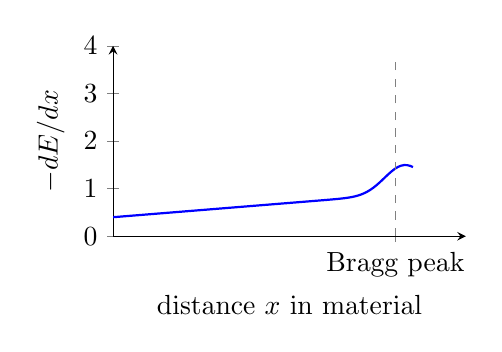
\begin{tikzpicture}
\begin{axis}[
  width=0.5\textwidth, height=4cm,
  xlabel={distance $x$ in material}, ylabel={$-dE/dx$},
  xmin=0, xmax=4, ymin=0, ymax=4,
  xtick={3.2}, xticklabels={Bragg peak},
  ytick={}, axis lines=left, samples=100,
]
  % Bragg curve: low then rapidly rising peak
  \addplot[thick,blue,domain=0:3.4]
    {0.4 + 0.15*x + 0.6*exp(-3*(x-3.3)^2/(0.3))} ;
  \draw[dashed,gray] (axis cs:3.2,0) -- (axis cs:3.2,3.8);
  \node[above,scale=0.8] at (axis cs:3.2,3.85) {stop};
\end{axis}
\end{tikzpicture}
\end{center}
\caption{Energy loss $-dE/dx$ (stopping power) as a function of depth $x$ in a material. The loss is relatively constant at first, then rises sharply to the \textbf{Bragg peak} just before the particle stops — exploited in proton therapy.}
\label{fig:bragg_peak}
\end{figure}

%%==========================================================================
\section{Central Force Potential Scattering (Recitation 15)}
%%==========================================================================

\textbf{IMPORTANT: MIGHT BE ON EXAM!}

\subsection{Setup}

\begin{figure}[H]
    \centering
    \caption{Central force scattering. The potential $U(r)$ is radially symmetric, so $\alpha_\text{left} = \alpha_\text{right}$.}
\end{figure}

\begin{itemize}
    \item Because $U(r)$ is radially symmetric, $\alpha_{\text{left}} = \alpha_{\text{right}}$.
    \item
    \[
        \frac{d\sigma}{d\Omega} = \frac{b}{\sin\theta}\left|\frac{db}{d\theta}\right|
    \]
    \item $\sigma_T \propto [\text{area}]$ --- effective cross section.
    \item Suppose:
    \[
        U = \begin{cases} \infty, & r < a \\ 0, & r > a \end{cases}
    \]
\end{itemize}

\begin{figure}[H]
    \centering
    \caption{Hard-sphere scattering geometry. The particle reflects off a hard sphere of radius $a$.}
\end{figure}

\[
    \theta = \pi - 2\phi \implies \phi = \tfrac{1}{2}(\pi - \theta)
\]
but $b = a\sin\phi = a\sin\!\left(\tfrac{1}{2}(\pi-\theta)\right) = a\cos\!\left(\tfrac{\theta}{2}\right)$.

\[
    \frac{d\sigma}{d\Omega}
    = \frac{b}{\sin\theta}\left|\frac{db}{d\theta}\right|
    = \frac{a\cos(\theta/2)}{\sin\theta}\cdot\left|-\frac{a}{2}\sin\!\left(\frac{\pi}{2}\right)\right|
    = \frac{a^2\sin(\theta/2)\cos(\theta/2)}{2\sin\theta}
    = \frac{a^2}{4}
\]

\[
    \sigma_T = \int d\sigma = \int\frac{a^2}{4}\,d\Omega
    = \iint\frac{a^2}{4}\sin\theta'\,d\theta'\,d\phi'
    = \frac{a^2}{4}\cdot 4\pi = \pi a^2,
\]
which is the ``impact area'' that the particle must hit.

\section{Central Force Potential}

\begin{enumerate}
    \item $\vect{F} = -\grad U(r) = -\dfrac{\partial U}{\partial r}\,\hat{r}$
    \item $\dfrac{d\vect{L}}{dt} = 0 \implies \vect{L} = \vect{r}\times\vect{p}$, $\vect{r}\perp\vect{L}$.
    \begin{itemize}
        \item $\mathcal{L} = \frac{1}{2}m(\dot{r}^2 + r^2\dot{\phi}^2) - U(r)$, $\phi$ is cyclic.
        \item $\implies mr^2\dot{\phi}$ is conserved.
        \item $E = K + U = \frac{1}{2}m(\dot{r}^2 + r^2\dot{\phi}^2) + U(r)$
        \[
            = \frac{1}{2}m\dot{r}^2 + \frac{mr^2\dot{\phi}^2}{2mr^2} + U(r)
            = \frac{1}{2}m\dot{r}^2 + \frac{\ell^2}{2mr^2} + U(r)
        \]
        \[
            E = \frac{1}{2}m\dot{r}^2 + U_{\text{eff}}(r)
        \]
        \[
            \dot{r} = \sqrt{\frac{2}{m}\bigl(E - U_{\text{eff}}(r)\bigr)}
        \]
        \[
            \int dr = \int\sqrt{\frac{2}{m}(E-U_{\text{eff}})}\,dt
        \]
    \end{itemize}
\end{enumerate}

\subsection{Stability of Circular Orbits}

\begin{itemize}
    \item $\dfrac{dU_{\text{eff}}}{dr} = 0$ (so you are at a local min of the potential)
    \item $\left.\dfrac{d^2 U_{\text{eff}}}{dr^2}\right|_{r=\rho} > 0$
    \item Note that $mr^2\dot{\phi} = \ell \implies \dfrac{\partial\phi}{\partial t} = \dfrac{\ell}{mr^2}$, so:
    \[
        \phi = \int\frac{\ell}{mr^2}\,dt = \int\frac{\ell}{mr^2}\,\frac{dr}{\sqrt{\dfrac{2}{m}(E-U_{\text{eff}})}}
    \]
\end{itemize}

\subsection*{Example: Conical Pendulum}

\begin{figure}[H]
    \centering
    \caption{Conical pendulum: mass $m$ on a string of length $\ell_0$ constrained to move on a cone of half-angle $\alpha$.}
\end{figure}

\[
    E = K + U = \frac{1}{2}m\dot{r}^2 + \frac{1}{2}\frac{\ell^2}{m(r\sin\alpha)^2} + mg
\]

\[
    t = \int dt = \int\sqrt{\frac{2}{m}(E-U_{\text{eff}})}\,\frac{dr}{\phantom{x}}
    = \int\frac{dr}{\sqrt{\dfrac{2}{m}\!\left(E - \dfrac{\ell^2}{2mr^2\sin^2\!\alpha} - mg\cos\alpha\right)}}
\]

\[
    \phi = \frac{\ell}{\sqrt{2m}\sin^2\!\alpha}\int\frac{dr}{r^2\sqrt{E - \dfrac{\ell^2}{2mr^2\sin^2\!\alpha} - mg\sin\alpha}}
\]

%%==========================================================================
\chapter{Principle Axes of Rotation and Rigid Body Motion}
%%==========================================================================

% Lec. 16, Wednesday January 29, 2025

\begin{itemize}
    \item Consider a 3D pendulum rotating at $\vec{\omega} = \omega\hat{z}$: in general $\vect{L} \neq I\vec{\omega}$.
\end{itemize}

\section{General Body: Inertia Tensor}

\begin{figure}[H]
    \centering
    \caption{A general rigid body rotating with $\vec{\omega} = \omega\hat{z}$. Each mass element $m_i$ is at position $\vect{r}_i$ with transverse distance $\rho_i$ from the rotation axis and axial coordinate $z_i$.}
\end{figure}

\begin{align*}
    \vect{L} &= \sum_i \vect{r}_i \times m_i\vect{v}_i
    = \sum_i m_i\,\vect{r}_i \times (\vec{\omega}\times\vect{r}_i) \\
    &= \sum_i m_i\!\left[(\vect{r}_i\cdot\vect{r}_i)\vec{\omega} - (\vect{r}_i\cdot\vec{\omega})\vect{r}_i\right]
\end{align*}

Using $r_i^2 = \rho_i^2 + z_i^2$ and $\vect{r}_i\cdot\vec{\omega} = z_i\omega$:

\[
    = \omega\sum_i m_i\!\left[(\rho_i^2 + z_i^2)\hat{z} - x_i z_i\,\hat{x} - y_i z_i\,\hat{y} - z_i^2\,\hat{z}\right]
\]

\[
    \implies \vect{L} = \omega\sum_i m_i\!\left[\rho_i^2\,\hat{z} - x_i z_i\,\hat{x} - y_i z_i\,\hat{y}\right]
\]

In general, the \textbf{inertia tensor} relates $\vect{L}$ and $\vec{\omega}$:

\[
    \begin{pmatrix} L_x \\ L_y \\ L_z \end{pmatrix}
    =
    \begin{pmatrix} I_{xx} & I_{xy} & I_{xz} \\ I_{yx} & I_{yy} & I_{yz} \\ I_{zx} & I_{zy} & I_{zz} \end{pmatrix}
    \begin{pmatrix} \omega_x \\ \omega_y \\ \omega_z \end{pmatrix}
\]

For the specific case $\omega_y = \omega_z = 0$:

\[
    \vect{L} = \begin{pmatrix} I_{xz}\,\omega \\ I_{yz}\,\omega \\ I_{zz}\,\omega \end{pmatrix}
\]

\[
    I_{zz} = \sum_i m_i\rho_i^2,\qquad
    I_{xz} = -\sum_i m_i x_i z_i = I_{zx},
    \quad\text{same for }I_{yz}\text{ but swap }x\leftrightarrow y.
\]

\textit{Example:} For two point masses A and B symmetrically placed, $I_{yz}^A = -myz$ and $I_{yz}^B = -m(-y)z$, so the off-diagonal terms cancel.

\begin{theorem}[Principal Axes]
There is a choice of axes (that does not rotate with the object) such that the inertia tensor is diagonal:
\[
    \overline{I} = \begin{pmatrix} I_1 & 0 & 0 \\ 0 & I_2 & 0 \\ 0 & 0 & I_3 \end{pmatrix}
\]
\end{theorem}

To find the principal axes: diagonalize the matrix
\[
    \begin{pmatrix} I_{xx} & I_{xy} & I_{xz} \\ I_{yx} & I_{yy} & I_{yz} \\ I_{zx} & I_{zy} & I_{zz} \end{pmatrix}
\]
The eigenvalues $\lambda_1, \lambda_2, \lambda_3$ become $I_1, I_2, I_3$.

\section{Torque and Euler's Equations}

\[
    \vect{T} = \dv{\vect{L}}{t} = \left(\dv{\vect{L}}{t}\right)_{\text{rot}} + \vec{\omega}\times\vect{L},
    \qquad \vect{v} = \vec{\omega}\times\vect{r}
\]

To see why, consider rotating the angular momentum components. After a small rotation $\Delta\theta_3$ about axis 3:

\[
    \Delta l_1 = -I_2\omega_2\,\Delta\theta_3,\quad
    \Delta l_2 = I_1\omega_1\,\Delta\theta_3,\quad
    \Delta l_3 = 0
\]

\[
    \dot{l}_1 = -I_2\omega_2\omega_3,\qquad
    \dot{l}_2 = I_1\omega_1\omega_3
    \quad\text{(think about where these appear)}
\]

\begin{formula}[Euler's Equations]
For the principal axes, $l_i = I_i\omega_i$ (directions labeled 1, 2, 3):
\[
    T_1 = I_1\dot{\omega}_1 + (I_3 - I_2)\omega_3\omega_2
\]
\[
    T_2 = I_2\dot{\omega}_2 + (I_1 - I_3)\omega_1\omega_3
\]
\[
    T_3 = I_3\dot{\omega}_3 + (I_2 - I_1)\omega_2\omega_1
\]
\end{formula}

\subsection{No Torque Situation}

Suppose $\omega_1 \gg \omega_2, \omega_3$, with $\omega_1$ constant.

\begin{enumerate}
    \item $I_1\dot{\omega}_1 = 0 \implies \omega_1 \approx \text{const}$
    \item $I_2\dot{\omega}_2 + (I_1 - I_3)\omega_1\omega_3 = 0$
    \item $I_3\dot{\omega}_3 + (I_2 - I_1)\omega_2\omega_1 = 0$
\end{enumerate}

Taking time derivatives (substituting equation 3 into the time derivative of equation 2):

\[
    I_2\ddot{\omega}_2 + (I_1-I_3)\omega_1\left(-\frac{(I_2-I_1)\omega_2\omega_1}{I_3}\right) = 0
\]

\[
    \ddot{\omega}_2 + \omega_2\omega_1^2\left[\frac{(I_1-I_3)(I_1-I_2)}{I_3 I_1}\right] = 0
    \quad\text{(const.)}
\]

If $(I_1-I_3)(I_1-I_2) > 0 \implies$ SHM with frequency:

\[
    \Omega_2 = \omega_1\sqrt{\frac{(I_1-I_3)(I_1-I_2)}{I_3 I_2}}
\]

Only if $I_1$ is max or min. If it isn't, then it isn't stable.

%%==========================================================================
\section{Rigid Body Motion (Recitation 16)}
%%==========================================================================

% Wednesday, January 29, 2025

\subsection{Angular Velocity with Euler Angles}

\begin{figure}[H]
    \centering
    \caption{Euler angles: $x,y,z$ are inertial coordinates; $x',y',z'$ are body axes. Three successive rotations: (1) rotate about $\hat{z}$ by $\phi$; (2) rotate about $\hat{x}'''$ by $\theta$; (3) rotate about $\hat{z}''$ by $\psi$.}
\end{figure}

\begin{itemize}
    \item $x,y,z \to$ inertial coordinates.
    \item $x',y',z' \to$ body axes.
    \item Rotation steps:
    \begin{enumerate}
        \item Rotate about $\hat{z}$: $\phi$
        \item Rotate about $\hat{x}'''$: $\theta$
        \item Rotate about $\hat{z}''$: $\psi$
    \end{enumerate}
    \item $\vect{r}' = U\vect{r} = U_\psi U_\theta U_\phi\,\vect{r}$ (Unitary transformation).
\end{itemize}

Rotation about 1 axis:
\[
    R_\alpha = \begin{pmatrix} \cos\alpha & \sin\alpha & 0 \\ -\sin\alpha & \cos\alpha & 0 \\ 0 & 0 & 1 \end{pmatrix}
\]

\begin{formula}[Euler Angle Transformation]
\[
    \vect{r}' =
    \begin{pmatrix} \cos\psi & \sin\psi & 0 \\ -\sin\psi & \cos\psi & 0 \\ 0 & 0 & 1 \end{pmatrix}
    \begin{pmatrix} 1 & 0 & 0 \\ 0 & \cos\theta & \sin\theta \\ 0 & -\sin\theta & \cos\theta \end{pmatrix}
    \begin{pmatrix} \cos\phi & \sin\phi & 0 \\ -\sin\phi & \cos\phi & 0 \\ 0 & 0 & 1 \end{pmatrix}
    \vect{r}
\]
\end{formula}

\[
    \vec{\omega} = \vec{\omega}_\phi + \vec{\omega}_\theta + \vec{\omega}_\psi
\]

\[
    \vec{\omega}_\phi = \dot{\phi}\,\hat{z} = U_\psi U_\theta\begin{pmatrix}0\\0\\\dot{\phi}\end{pmatrix}
    = \begin{pmatrix}\dot{\phi}\sin\theta\sin\psi \\ \dot{\phi}\sin\theta\cos\psi \\ \dot{\phi}\cos\theta\end{pmatrix}
    = \dot{\phi}(\sin\theta\sin\psi\,\hat{x}' + \sin\theta\cos\psi\,\hat{y}' + \cos\theta\,\hat{z}')
\]

\[
    \vec{\omega}_\theta = \dot{\theta}\,\hat{x}''' = U_\psi\begin{pmatrix}\dot{\theta}\\0\\0\end{pmatrix}
    = \begin{pmatrix}\dot{\theta}\cos\psi \\ -\dot{\theta}\sin\psi \\ 0\end{pmatrix}
    = \dot{\theta}(\cos\psi\,\hat{x}' - \sin\psi\,\hat{y}')
\]

\[
    \vec{\omega}_\psi = \dot{\psi}\,\hat{z}'' = \dot{\psi}\,\hat{z}'
    \quad\text{(inertial coordinates)}
\]

Thus in the body axes frame:
\[
    \vec{\omega} = \hat{x}'(\dot{\phi}\sin\theta\sin\psi + \dot{\theta}\cos\psi)
                + \hat{y}'(\dot{\phi}\sin\theta\cos\psi - \dot{\theta}\sin\psi)
                + \hat{z}'(\dot{\psi}\cos\theta + \dot{\phi})
\]

\subsection{Example: Point Mass on a Disc}

\begin{figure}[H]
    \centering
    \caption{A disc of radius $R$ and total mass $M$ (with surface mass density $\sigma = M/\pi R^2$) with a point mass $m = 3M/8$ at radius $R$ from center (point B), with the axis at point A.}
\end{figure}

\textbf{Inertia Tensor of the disc alone:}

\[
    I_{zz} = \int\sigma(x^2+y^2)\,dA = \int_0^R \sigma r^2(2\pi r\,dr) = \frac{1}{2}MR^2
\]
\[
    I_{xx} = \int\sigma y^2\,dA = \frac{1}{2}\int\sigma(x^2+y^2)\,dA = \frac{MR^2}{4}
\]
\[
    I_{yy} = \frac{MR^2}{4},\qquad I_{xy} = I_{yz} = I_{xz} = 0
\]

\[
    \implies I_{\text{disk}}^{\text{center}} = \frac{MR^2}{4}\begin{pmatrix}1&0&0\\0&1&0\\0&0&2\end{pmatrix}
\]

By the parallel axis theorem (shifting to point A):
\[
    \frac{MR^2}{4}\begin{pmatrix}1&0&0\\0&1&0\\0&0&2\end{pmatrix}
    + MR^2\begin{pmatrix}0&0&0\\0&1&0\\0&0&1\end{pmatrix}
    = \frac{MR^2}{4}\begin{pmatrix}1&0&0\\0&5&0\\0&0&6\end{pmatrix}
\]

\textbf{Inertia tensor of the point mass at B} (about A), using $I_{ab}^A = m(\delta_{ab}r^2 - r_a r_b)$:

\[
    I_{xx} = m(y^2+z^2) = mR^2,\quad
    I_{yy} = m(x^2+z^2) = mR^2,\quad
    I_{zz} = m(x^2+y^2) = 2mR^2
\]
\[
    I_{xy} = I_{yx} = -mxy = -mR^2,\quad
    I_{xz} = I_{zx} = I_{yz} = I_{zy} = 0
\]

\[
    I_{\text{point mass}}^A = \frac{3M}{8}R^2\begin{pmatrix}1&-1&0\\-1&1&0\\0&0&2\end{pmatrix}
\]

\textbf{Combined inertia tensor:}
\[
    I_{\text{combined}} = I_{\text{disk}}^A + I_{\text{point mass}}^A
    = \frac{MR^2}{8}\begin{pmatrix}13&-3&0\\-3&7&0\\0&0&18\end{pmatrix}
\]

\textbf{Finding principal axes:} Solve $I\,\vec{\xi} = \lambda\,\vec{\xi}$:

\[
    I_1 = \frac{9}{4}MR^2,\quad \vec{\xi}_1 = \begin{pmatrix}0\\0\\1\end{pmatrix} \sim \hat{z}
\]
\[
    I_2 = \frac{1}{2}MR^2 \implies \vec{\xi}_2 = \frac{1}{\sqrt{10}}\begin{pmatrix}1\\3\\0\end{pmatrix} \sim \hat{x}+3\hat{y}
\]

(Third eigenvalue $I_3$ not completed in notes.)

%%==========================================================================
\chapter{Action-Angle Variables}
%%==========================================================================

% Thursday, January 30, 2025

\section{Canonical Transformation: $q,p,h \to Q,P,H$}

\begin{itemize}
    \item Any coordinate-coordinate transformation is canonical.
    \item Consider Hamiltonians where $\pdv{h}{t} = 0$ and where $h(q,p) \to H(P)$:
    \[
        \implies \dot{P} = -\pdv{H}{Q} = 0 \implies P\text{ conserved}
    \]
    \[
        \dot{Q} = \pdv{H}{P} = \text{constant} \equiv \alpha \implies Q(t) = \alpha t + Q_0
    \]
    \item Recall generator functions $F(q,P) \equiv W(q,P)$:
    \[
        h = \frac{p^2}{2m} + U(q) = E
    \]
    \[
        p = \pm\sqrt{2m(E-U(q))}
    \]
\end{itemize}

\section{Action-Angle Principle}

\begin{figure}[H]
\begin{center}
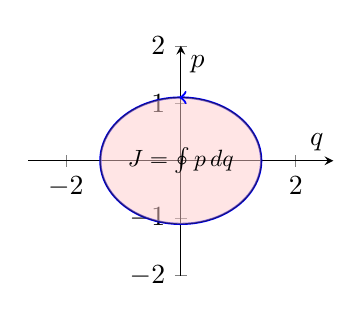
\begin{tikzpicture}
\begin{axis}[
  width=0.45\textwidth, height=4.5cm,
  xlabel={$q$}, ylabel={$p$},
  xmin=-2, xmax=2, ymin=-2, ymax=2,
  xtick={}, ytick={},
  axis lines=center, axis equal,
]
  % Closed ellipse = phase-space orbit
  \addplot[thick,blue,domain=0:360,samples=100]
    ({1.4*cos(x)}, {1.1*sin(x)});
  % Shade the interior
  \addplot[fill=red!20,opacity=0.5,domain=0:360,samples=100]
    ({1.4*cos(x)}, {1.1*sin(x)}) -- cycle;
  % Arrow on orbit
  \addplot[thick,blue,->,domain=89:91,samples=5]
    ({1.4*cos(x)}, {1.1*sin(x)});
  % Action area label
  \node[scale=0.85] at (axis cs:0,0) {$J = \oint p\,dq$};
\end{axis}
\end{tikzpicture}
\end{center}
\caption{Phase-space orbit for a bound periodic system. The trajectory is a closed curve in the $(q,p)$ plane; the enclosed area (red shading) equals the action variable $J = \oint p\,dq$, which is an adiabatic invariant.}
\label{fig:phase_space_orbit}
\end{figure}

\[
    p = \pdv{W}{q},\qquad Q = \pdv{W}{P}
    \quad\text{(comes from }F\text{)}
\]

\begin{itemize}
    \item Notice that the area (red) $= P = \oint p\,dq = \text{const}$.
    \item Let $\delta Q = \dfrac{\partial Q}{\partial q}\delta q + \dfrac{\partial Q}{\partial P}\delta P \bigg|_{\to 0}$:
    \begin{align*}
        \Delta Q\big|_{\text{1 period}}
        &= \oint\pdv{Q}{q}\,\delta q
        = \oint\frac{\partial^2 W}{\partial P\,\partial q}\,dq
        = \pdv{}{P}\oint\pdv{W}{q}\,dq \\
        &= \pdv{}{P}\oint p\,dq = 1
        \implies Q\text{ changes at a rate of 1 unit/period}
    \end{align*}
    \item Thus $\Delta Q = 1 = \alpha T$:
    \[
        \boxed{\alpha = \frac{1}{T}}
    \]
    \item But $\alpha = \pdv{H}{P} = \pdv{E}{P}$, and because energy is conserved:
    \[
        \boxed{T = \pdv{P}{E}}
    \]
\end{itemize}

\begin{formula}[Action-Angle Variables]
In action-angle formalism, $P \equiv J = \oint p\,dq$ (essentially the value of the reduced action, but for a fixed path). Then:
\[
    Q(t) = \pdv{E}{J}\,t + Q_0,\qquad Q \equiv \theta
\]
\[
    \alpha = \nu = \pdv{E}{J},\qquad T = \pdv{J}{E}
\]
\end{formula}

\subsection{Example: SHO}

\begin{figure}[H]
    \centering
    \caption{Ellipse traced by the SHO in phase space. The area $J = \pi ab$ is the action variable.}
\end{figure}

\begin{itemize}
    \item $h = \dfrac{p^2}{2m} + \dfrac{1}{2}kx^2 = E$
    \item In phase space: $\dfrac{x^2}{a^2} + \dfrac{p^2}{b^2} = 1$
    \item We know that $J = \text{area} = \pi ab$:
    \[
        = \pi\sqrt{2mE}\cdot\sqrt{\frac{2E}{k}} = 2\pi E\sqrt{\frac{m}{k}}
    \]
    \item $T = \pdv{J}{E} = 2\pi\sqrt{\dfrac{m}{k}} = \dfrac{2\pi}{\omega}$
    \item To find $Q$: $\phi(t) = 2\pi\cdot\dfrac{\omega}{2\pi} = \omega t$
\end{itemize}

\subsection{Cycloid Problem}

\begin{figure}[H]
    \centering
    \caption{Shape of the well formed by a cycloid (parametrized by $\phi$). The potential is zero at the top of the cycloid.}
\end{figure}

\begin{itemize}
    \item $X(\phi) = R(\phi + \sin\phi)$, $Y(\phi) = -R\cos\phi$
    \item Start at $\phi(0) = \phi_0$, $\dot{\phi}(0) = 0$; how long does it take to get to the bottom?
\end{itemize}

\[
    \dot{X} = R(\dot{\phi} + \cos\phi\,\dot{\phi}),\quad \dot{Y} = R\sin\phi\,\dot{\phi}
\]
\[
    V^2 = \dot{X}^2 + \dot{Y}^2 = R^2\dot{\phi}^2(1 + \cos^2\phi + 2\cos\phi + \sin^2\phi)
    = 2R^2\dot{\phi}^2(1+\cos\phi)
\]

\[
    L = mR^2\dot{\phi}^2(1+\cos\phi) + mgR(\cos\phi - 1)
\]
\[
    = mR^2\dot{\phi}^2\cdot 2\cos^2\frac{\phi}{2} - mgR\cdot 2\sin^2\frac{\phi}{2}
    = 2mR^2\dot{\phi}^2\cos^2\frac{\phi}{2} - 2mgR\sin^2\frac{\phi}{2}
\]

\[
    p = \pdv{L}{\dot{\phi}} = 4mR^2\dot{\phi}\cos^2\frac{\phi}{2}
\]

Notice that $p\dot{\phi} = 2K$.

\[
    H = p\dot{\phi} - L = 2mR^2\cos\frac{\phi}{2}\cdot\frac{p^2}{\underbrace{16m^2R^4\cos^4(\phi/2)}} + 2mgR\sin^2\frac{\phi}{2} = E
\]
\[
    = \frac{p^2}{8mR^2\cos^2\!\frac{\phi}{2}} + 2mgR\sin^2\frac{\phi}{2} = 2mgR\sin^2\frac{\phi}{2}
\]

\[
    \implies p^2 = 8mR^2\cos^2\frac{\phi}{2}\left[2mgR\!\left(\sin^2\frac{\phi_0}{2} - \sin^2\frac{\phi}{2}\right)\right]
\]

\[
    J = \oint p\,d\phi = 4\int_0^{\phi_0} p\,d\phi
    = 16mR^{3/2}\sqrt{g}\int_0^{\phi_0}d\phi\cos\frac{\phi}{2}\sqrt{\sin^2\frac{\phi_0}{2} - \sin^2\frac{\phi}{2}}
\]

(Make sure the integral is positive.)

Substitution: $z = \sin\dfrac{\phi}{2}$, $dz = \cos\dfrac{\phi}{2}\dfrac{d\phi}{2}$, $z_0 = \sin\dfrac{\phi_0}{2}$:

\[
    J = 16mR^{3/2}\sqrt{g}\int_0^{z_0} 2\,dz\sqrt{z_0^2 - z^2}
\]

\[
    = 16mR^{3/2}\sqrt{g}\left[z_0^2\sin^{-1}\!\left(\frac{z}{z_0}\right) + z\sqrt{z_0^2-z^2}\right]_0^{z_0}
    = z_0^2\frac{\pi}{2} - 0 - 0
    = \frac{\pi}{2}\sin^2\frac{\phi_0}{2}
\]

\[
    J = 16mR^{3/2}\sqrt{g}\cdot\frac{\pi E}{4mgR} = 4\pi E\sqrt{\frac{R}{g}}
\]

\[
    T = \pdv{J}{E} = 4\pi\sqrt{\frac{R}{g}} \implies \boxed{\text{time to bottom is }\pi\sqrt{\frac{R}{g}}}
\]

%%==========================================================================
\chapter{Final Summary}
%%==========================================================================

% Thursday, January 30, 2025

\section{Constrained Motion}

\section{Final Exam Review (Recitation 17)}

\[
    \mathcal{L}(q,\dot{q},t) = K(\dot{q},t) - U(q,t)
\]

\textbf{EOM:}
\[
    \dv{t}\!\left(\pdv{\mathcal{L}}{\dot{q}}\right) - \pdv{\mathcal{L}}{q} = 0
\]

\subsection{If Constraints:}

\subsubsection{(1) Holonomic Constraints}

No $\dot{q}$ dependence $\implies f_\alpha^{\text{index of constraint}}(\vec{q}, t) = 0$.

E.g.\ motion restricted to specific surfaces:
\[
    r^2 - (x^2 + y^2) = 0\quad\text{(cone)}
\]

\begin{formula}[Generalized Forces]
\[
    F_\alpha(\vec{q},t) = \lambda_\alpha\,\pdv{f_\alpha}{q_a}
\]
\end{formula}

\[
    \dv{t}\!\left(\pdv{\mathcal{L}}{\dot{q}_i}\right) - \pdv{\mathcal{L}}{q_i}
    = \sum_\alpha \lambda_\alpha\,\pdv{f_\alpha}{q_i}
\]

\subsubsection{(2) Semi-Holonomic}

Linear dependence on $\dot{q}$:

\begin{formula}[Semi-Holonomic Constraint]
\[
    f = \sum_i a_i(q_i, t)\,\dot{q}_i + B(q_i, t) = 0
\]
\[
    f = \dv{t}\!\bigl(g(q_i,t)\bigr),\quad\text{where }a_i = \pdv{g}{q_i},\quad B = \pdv{g}{t}
\]
\end{formula}

\textbf{Conditions:} Because $\dfrac{\partial g}{\partial q_i\,\partial t} = \dfrac{\partial^2 g}{\partial t\,\partial q_i}$:
\begin{enumerate}
    \item $\pdv{a_i}{t} = \pdv{B}{q_i}$
    \item $\pdv{a_i}{q_j} = \pdv{a_j}{q_i}$
\end{enumerate}

\[
    \text{EOM:}\quad\dv{t}\!\left(\pdv{\mathcal{L}}{\dot{q}_i}\right) - \pdv{\mathcal{L}}{q_i}
    = \sum_\alpha \lambda_\alpha\,\partial f_\alpha
\]

\subsection{Hamiltonian}

\textit{Last-minute question: when is the Hamiltonian $=$ energy $= K+U$?}

\begin{formula}[Hamiltonian]
\[
    H(q,p,t) = \sum_i p_i\dot{q}_i - \mathcal{L}(q,\dot{q},t),\quad\text{where }p_i \equiv \pdv{\mathcal{L}}{\dot{q}_i}
\]
\end{formula}

\textbf{EOM:}
\[
    \pdv{H}{p_i} = \dot{q}_i,\qquad
    \pdv{H}{q_i} = -\dot{p}_i,\qquad
    \pdv{H}{t} = -\pdv{\mathcal{L}}{t}
\]

In order for $H = E$, there must be no explicit time dependence.

\subsection{Non-Hamiltonian Forces}

They can be added as such:
\[
    \dot{p}_i = -\pdv{H}{q_i} + F_i
\]

\subsection{Poisson Brackets}

\[
    [f,g] = \sum_k\left(\pdv{f}{q_k}\pdv{g}{p_k} - \pdv{f}{p_k}\pdv{g}{q_k}\right)
\]

Check if a quantity is conserved:
\begin{formula}[Time Evolution via Poisson Bracket]
\[
    \boxed{\dv{f}{t} = \pdv{f}{t} + [f, H]}
\]
\end{formula}

\subsubsection{Canonical Coordinate Transformation Requirements}

To show that $q\to Q$, $p\to P$ is canonical, you need to show that $[Q_i, Q_k]_{q,p}$, $[Q_i, Q_i]_{q,p}$, $[P_i, P_k]_{q,p}$ satisfies (1), (2), (3):

\begin{enumerate}
    \item $[q_i, q_k] = 0$
    \item $[p_i, p_k] = 0$
    \item $[q_i, p_k] = \delta_{ik}$
\end{enumerate}

\subsubsection{Useful Identities}

\begin{enumerate}
    \item $[q_i, q_j]_{q,p} = [p_i, p_j]_{q,p} = 0$
    \item $[q_i, p_j]_{q,p} = \delta_{ij}$
    \item $[F, G] = -[G, F]$
\end{enumerate}

With the Hamiltonian:
\begin{enumerate}
    \item $[q, H] = \dot{q}$
    \item $[p, H] = \dot{p}$
\end{enumerate}

\begin{fact}[Conservation via Poisson Brackets]
If $[F,H] = [G,H] = 0$ (i.e., $F$ and $G$ are conserved), then $[F,G]$ is also conserved.

\textit{Example:} Angular momentum can only be conserved for 1 or 3 axes.
\end{fact}

\begin{formula}[Poisson Brackets Invariant Under Canonical Transformations]
\[
    [F,G]_{p,q} = [F,G]_{P,Q}
\]
\end{formula}

\section{Generating Canonical Transformations}

We want to find a function $F(q,P,t)$ such that:
\begin{formula}[Generator Function]
\[
    \boxed{p = \pdv{F}{q},\qquad Q = \pdv{F}{P},\qquad H = h + \pdv{F}{t}}
\]
\end{formula}

\begin{enumerate}
    \item Find the transformed Hamiltonian $H$.
    \item Find the equations of motion and solve.
    \item Transform back to original coordinates $q,p$.
\end{enumerate}

\section{Infinitesimal Canonical Transformations}

For $F$'s of the form $F = qP + \varepsilon f(q,P)$ for $\varepsilon$ small:
\[
    p = \pdv{F}{q},\qquad Q = \pdv{F}{P}\quad\text{as usual}
\]

But now:
\begin{enumerate}
    \item If $f(q,p) = h(q,p) \implies$ \textbf{Hamiltonian generates time-translation!}
    \begin{itemize}
        \item e.g.\ $p = p(t+\delta t)$, $Q = q(t+\delta t)$ (regardless of whether $E$ is conserved).
    \end{itemize}
    \item If $F(q,p) = qP + \delta q\,p \implies$ \textbf{Momentum is always the generator of space translation!}
    \item \textbf{Angular momentum is the generator of rotations!}
\end{enumerate}

\section{Liouville's Theorem}

\begin{itemize}
    \item Continuity equation: $\pdv{\varrho}{t} + \grad\cdot\vect{J} = 0$
    \item The density of states in an ensemble of identical states with different initial conditions is constant along every trajectory in phase space, NOT at any fixed point $\left(\pdv{\varrho}{t} = 0\right)$.
    \item \textbf{Important:} For a non-Hamiltonian force $F$, the Liouville equation becomes:
    \[
        \pdv{\varrho}{t} + \sum_i\pdv{F_i}{p_i}\,\varrho = 0
    \]
    \item If $F$ is divergence-free with respect to momentum space $\left(\sum_i\pdv{F_i}{p_i} = 0\right)$, then $\pdv{\varrho}{t} = 0$.
    \item Canonical transformations preserve phase space volumes!
\end{itemize}

%%==========================================================================
\section{Scattering (Summary)}
%%==========================================================================

\begin{figure}[H]
    \centering
    \caption{Scattering summary diagram. A particle with initial momentum $\vect{p}_i$ and impact parameter $b$ scatters off a potential centered at the origin through angle $\theta$. The solid angle element $d\Omega$ subtended by the scattered ring is shown.}
\end{figure}

\begin{itemize}
    \item $\theta$ (scatter angle): direction between initial and final $\vect{p}$.
    \item $b$: impact parameter, $b = R\sin\alpha$.
    \item $\alpha$: angle from origin to point of closest approach.
    \item \textbf{Important:} If the potential has azimuthal symmetry, the trajectory of the particle obeys time-translation symmetry $\implies$
    \[
        \boxed{\theta = \pi - 2\alpha}
    \]
\end{itemize}

\subsection{Differential Cross Section}

\[
    \int\frac{d\sigma}{d\Omega}\,d\Omega = \sigma_T \propto [\text{area}]
    = \frac{\text{total scattering rate}}{L}
    \quad\left(\frac{\#\text{ particles}}{\text{[time][area]}}\right)
\]

\[
    \implies \left(\frac{d\sigma}{d\Omega}\right)\Delta\Omega\text{ is scattering rate through }\Delta\Omega\text{ divided by }L
\]

\[
    d\Omega = \sin\theta'\,d\theta'\,d\phi = 2\pi\sin\theta'\,d\theta'
    \implies \int d\Omega = 4\pi
\]

If $b(\theta)$ is 1-to-1, then the rate of beam particles in $[b,\Delta b]$ equals the rate of particles scattering through $d\Omega$:

\begin{formula}[Differential Cross Section]
\[
    \boxed{\frac{d\sigma}{d\Omega} = \frac{b}{\sin\theta}\left|\frac{db}{d\theta}\right|}
\]
\end{formula}

\subsection{Calculating Mean Free Path}

\begin{itemize}
    \item Enter rest frame of the particle.
    \item Suppose potential wells have a density of $\rho_U$.
    \item Suppose beam velocity is $v_n$.
    \item The luminosity of the beam is $= \rho v_n$.
    \item Thus the mean free path:
    \[
        D = \frac{v_n}{L\sigma} = \frac{v_n}{\rho\,v_n} = \frac{1}{\rho\,\sigma}
    \]
\end{itemize}

\subsection{Handy Formula: Central Potential}

If $U$ is a central potential, angular momentum is conserved:
\[
    E = \frac{1}{2}m\dot{r}^2 + \frac{\ell^2}{2mr^2} + U(r),\qquad
    \ell^2 = (bp_0)^2 = b^2\cdot 2mE_0
\]

Circular orbit is stable when $\dfrac{dU_{\text{eff}}}{dr} = 0$ and $\left.\dfrac{d^2U_{\text{eff}}}{dr^2}\right|_{r=\rho} > 0$.

\section{Rigid-Body Motion (Summary)}

\begin{itemize}
    \item There is a choice of axes such that the inertia tensor is diagonal.
    \item If $\omega_1 \gg \omega_2, \omega_3$, the rotation is only stable if $I_1$ is a \underline{minimum} or \underline{maximum}.
    \item Frequency for SHM:
    \[
        \Omega_2 = \omega_1\sqrt{\frac{(I_1-I_3)(I_1-I_2)}{I_3 I_2}}
    \]
\end{itemize}

%%==========================================================================
\section{Examples}
%%==========================================================================

\subsection{Canonical Transformation Example}

\begin{example}[Verifying Canonical Transformation]
Let $Q = p + iaq$, $P = \dfrac{p - iaq}{2ia}$.

Want to show (WTS) $[Q,Q]_{q,p} = 0$:
\[
    [Q,Q] = \pdv{Q}{q}\pdv{Q}{p} - \pdv{Q}{p}\pdv{Q}{q} = 0
\]
$[P,P]_{q,p} = 0$: same as above.

$[Q,P] = 1$:
\[
    [Q_1, P] = \pdv{Q}{q}\pdv{P}{p} - \pdv{Q}{p}\pdv{P}{q}
    = ia\cdot\frac{1}{2ia} - 1\cdot\left(-\frac{ia}{2ia}\right)
    = \frac{1}{2} + \frac{1}{2} = 1\checkmark
\]
\end{example}

\subsection{Constraints Example: Hoop Rolling on a Cylinder}

\begin{figure}[H]
    \centering
    \caption{A hoop of mass $m$ and radius $r$ rolling without slipping on a cylinder of radius $R$. The hoop starts from rest on top of the cylinder.}
\end{figure}

\begin{itemize}
    \item Hoop rolls without slipping on the cylinder.
    \item Starts from rest on top of the cylinder.
    \item Rolling without slipping --- write ALL constraints!
    \[
        g_1 = \dot{\rho} = 0,\quad \rho = R + r\quad\text{(semi-holonomic)}
    \]
    \[
        g_2 = \rho\dot{\theta} - r\dot{\phi} = 0
    \]
\end{itemize}

\[
    L = \frac{m}{2}(\dot{\rho}^2 + \rho^2\dot{\theta}^2) + \frac{m}{2}r^2\dot{\phi}^2 - mg\rho\cos\theta
    \quad (I_{\text{hoop}} = mr^2)
\]

Equations of motion with generalized forces:

\begin{align*}
    \rho:&\quad\dv{t}\!\left(\pdv{L}{\dot{\rho}}\right) - \pdv{L}{\rho} - \sum_i\lambda_i\pdv{g_i}{\dot{\rho}} = 0\\
    &\implies m\ddot{\rho} - m\rho\dot{\theta}^2 + mg\cos\theta - \lambda_1 = 0\\[6pt]
    \theta:&\quad\dv{t}\!\left(\pdv{L}{\dot{\theta}}\right) - \pdv{L}{\theta} - \sum_i\lambda_i\pdv{g_i}{\dot{\theta}} = 0\\
    &\implies \dv{t}(m\rho^2\dot{\theta}) - mg\rho\sin\theta - \lambda_2\rho = 0\\[6pt]
    \phi:&\quad\dv{t}\!\left(\pdv{L}{\dot{\phi}}\right) - \pdv{L}{\phi} - \sum_i\lambda_i\pdv{g_i}{\dot{\phi}} = 0\\
    &\implies mr^2\ddot{\phi} + \lambda_2 r = 0
\end{align*}

\[
    F_\rho = \sum_i\lambda_i\pdv{g_i}{\dot{\rho}} = \lambda_1 = 0
    \implies \text{no force on the contact point}
\]

From the $\phi$ equation: $\lambda_2 = -mr\ddot{\phi} = -mr\ddot{\theta}$ (since $\rho\dot{\theta} = r\dot{\phi}$ implies $\dot{\phi} = \dot{\theta}$ for $\rho = R+r \approx R$).

From the $\theta$ equation:
\[
    \dv{t}(m\rho^2\dot{\theta}) - mg\rho\sin\theta - \rho\lambda_2 = 0
\]
\[
    2m\rho\dot{\rho}\dot{\theta} + m\rho^2\ddot{\theta} - mg\rho\sin\theta - \rho\lambda_2 = 0
\]

Since $\dot{\rho} = 0$:
\[
    \implies \boxed{\ddot{\theta} = \frac{g\sin\theta}{2\rho}}
\]

Solve this to get $\dot{\theta}^2 = \dfrac{g}{\rho}(1 - \cos\theta)$.

Plug into EOM for $\rho$ to get $\ddot{\rho} = 0$:
\[
    \lambda_1 = mg(2\cos\theta - 1) = 0 \implies \boxed{\theta = \frac{\pi}{3}}
\]
